\section{Technischer Bericht}

\subsection{Einleitung und Übersicht}


\subsection{Methode 635} \label{subsec:methode_635_desc}
Die gesamte Beschreibung der Methode 635 wurde von \href{https://kreativitätstechniken.info/6-3-5-methode/}{kreativitästechniken.info} übernommen.


Die 635-Methode (auch Methode 6-3-5 geschrieben) ist eine Brainwriting-Kre\-ati\-vi\-täts\-technik. Der Name der Methode leitet sich aus den drei wesentlichen Eigenschaften der Methode ab: 6 Teilnehmer erhalten jeweils ein Blatt, auf dem sie 3 Ideen notieren und die Blätter dann insgesamt 5 mal weiterreichen.

\subsubsection*{Anwendungsgebiete der Methode 635}
Die 635-Methode ist eine Variante des Brainwriting. Sie eignet sich für die erste Phase im kreativen Prozess. Mit ihrer Hilfe werden Ideen gesammelt ohne dass eine Bewertung stattfindet. In kurzer Zeit können im Idealfall 108 Ideen entstehen. Die Aufforderung, bestehende Ideen aufzugreifen und weiterzuentwickeln macht die 635-Methode zu einer konstruktiven Kreativitätstechnik. Gleichzeitig kann die strukturierte Form jedoch auch die Kreativität bremsen. In der Praxis entstehen daher oft etwas weniger Ideen.

\subsubsection*{Vorgehen bei der Methode 635}
Der Moderator erklärt zunächst die Regeln der 635-Methode, führt die Teilnehmer in das Ausgangsproblem ein und ist im Folgenden für die Zeitmessung verantwortlich. Sobald die Teilnehmer über die Ausgangsfrage oder -problem aufgeklärt sind, startet die erste von sechs Runden. In jeder Runde werden die Teilnehmer aufgerufen, die oberste noch freie Zeile, bestehend aus 3 Kästchen, mit ihren Ideen zu füllen. Dabei sollten die Teilnehmer die Ideen der Vorgänger aufgreifen, erweitern und/oder weiterentwickeln. Nach einer festgelegten Zeit von beispielsweise 5 Minuten beendet der Moderator die Runde. Die Teilnehmer reichen ihr Arbeitsblatt im Uhrzeigersinn an ihren Sitznachbarn weiter und eine neue Runde beginnt. Im Idealfall sind nach 6 Runden genau 6*18 = 108 Ideen entstanden. In der Praxis ist die Anzahl aufgrund von doppelten oder leeren Einträgen wahrscheinlich etwas geringer. Dennoch sollten nun zahlreiche Ideen vorliegen.


Nun kann eine Diskussion, Analyse und Bewertung der Ideen erfolgen.

\newpage

% Hier soll beschrieben werden wie der technische Bericht aufgebaut ist und was die Kapitel beinhalten.

\subsection{Vorstudie}
In der Vorstudie beschäftigten wir uns zuerst mit der Methode 635 an sich, um ein Gefühl dafür zu bekommen, wie es ist, diese selbst an einem konkreten Problem zu nutzen. 

Weiter beschäftigten wir uns mit Xamarin. Hierbei war vor allem der Entscheid zwischen Xamarin.Forms und Xamarin native von grosser Bedeutung, da dieser im späteren Projektverlauf kaum mehr rückgängig zu machen ist.

Ein weiterer Teil der Vorstudie bestand darin eine passende Umgebung  für das automatische Deployen der Xamarin Applikation zu finden. 

Zum Schluss der Vorstudie beschäftigten wir uns mit der Frage, welches Backend wir für unser Projekt verwenden sollten.

Einige wichtige Punkte und Entscheide waren stark von der Vorstudie abhängig.Es war daher entscheidend, bei der Vorstudie sorgfältig zu arbeiten.


\subsubsection{Erste Erfahrungen mit der Methode 635} \label{subsub:erste_erfahrungen_mit_methode_635}
Bevor wir uns mit den technischen Details der Umsetzung zur Cross-Plattform App auseinander gesetzt haben, spielte jeder der beiden Projektmitgliedern die Methode 635, wie in Kapitel \ref{subsec:methode_635_desc} beschrieben, mit seiner Familie, Bekannten oder Freunden einmal durch. 

Dabei wurden folgende persönliche Erfahrungen und Beobachtungen gemacht:

\begin{description}[leftmargin=!,labelwidth=\widthof{\bfseries Interessante Methode}]
	\item[Diskussion gestartet] Schon nach 2-3 Runden konnte beobachtet werden, dass sich spannende Diskussionen zum gestellten Problem entwickelten. Die Teilnehmer mussten sogar angehalten werden die Diskussionen auf dem Papier weiterzuführen, da sonst die Aussagen verloren gehen.
	\item[Interessante Methode] Die Teilnehmer empfanden die Methode 635 als spannend und interessant. Durch die einzelnen Teilnehmer waren auch verschiedenste Blickwinkel auf das Problem vertreten, was wiederum zu unterschiedlichsten neuen Ideen führe.
	\item[Wertung einführen] Was allerdings als kleiner Nachteil empfunden wurde, war der Umstand, dass die Methode 635 in der original Version keine Möglichkeit für Wertungen bietet. 
	
	Als Mensch bildet man sich während des Lesens der einzelnen Ideen automatisch eine Meinung darüber und wird dadurch stark dazu verleitet, eine wertende Bemerkung statt einer neuen oder angepassten Idee zu schreiben.
	
	Eine mögliche Verbesserung könnte darin bestehen, ein Möglichkeit für Wertungen der Ideen einzuführen. Dies könnte so aussehen, dass man neben dem Text auch ein Label (z.B. Pro oder Contra) und die Idee, welche man bewerten will, auswählen kann.
\end{description}

\subsubsection{Xamarin.Forms oder Xamarin native?}
%TODO würde hier die Vorteile und Nachteile von Forms und native zueinander erklären. Die Begründung warum wir uns für das eine entschieden haben, würde ich allerdings ins Architekturentscheide nehmen -> daher auch gleicher Titel im Dokument Architekturentscheide.

\subsubsection{Visual Studio App Center}


\subsubsection{Backend-Technologie}
Das Play Framework \cite{PlayFramework} ist ein, unter der Apache 2 Lizenz stehendes, Web Application Framework. Es folgt dem MVC-Pattern und erleichtert das Erstellen von Webanwendungen. Durch den Aufbau ermöglicht es dem Entwickler unter anderem auf einfache Art und Weise eine RESTful API zu schreiben. 

Play basiert auf einer zustandslosen und schlanken Architektur. Da es auf Akka aufgebaut ist, nützt es eine vollständig asynchrones I/O. Ausserdem bietet Play minimalen Ressourcenverbrauch. 

Sobald am Code eine Änderung vorgenommen wurde, wird der Server automatisch neugestartet, was die Produktivität des Entwicklers  weiter erhöht.

Jeglicher Code, welcher nicht kompiliert werden konnte, wird zudem im Browser angezeigt und man weiss als Entwickler sofort auf welcher Zeile man nachbessern muss. 

Seit der Version 2.0 des Play Frameworks ist der Framework Core in Scala geschrieben und als Build Tool wird SBT verwendet. Für das Testen stehen verschiedene Test Frameworks sowohl für Java als auch für Scala zur Verfügung. Mittels Scalatest oder JUnit können Unit Tests für beide Sprachen geschrieben werden. Es ist auch möglich Tools wie scoverage für die Code Coverage zu verwenden. 

\newpage

\subsection{Anforderungsspezifikation}

\subsubsection{Funktionale Anforderungen}

\paragraph{Brief Use-Cases}

Im Folgenden ist das Use-Case-Diagramm dargestellt.
\begin{figure}[h]
	\centering
	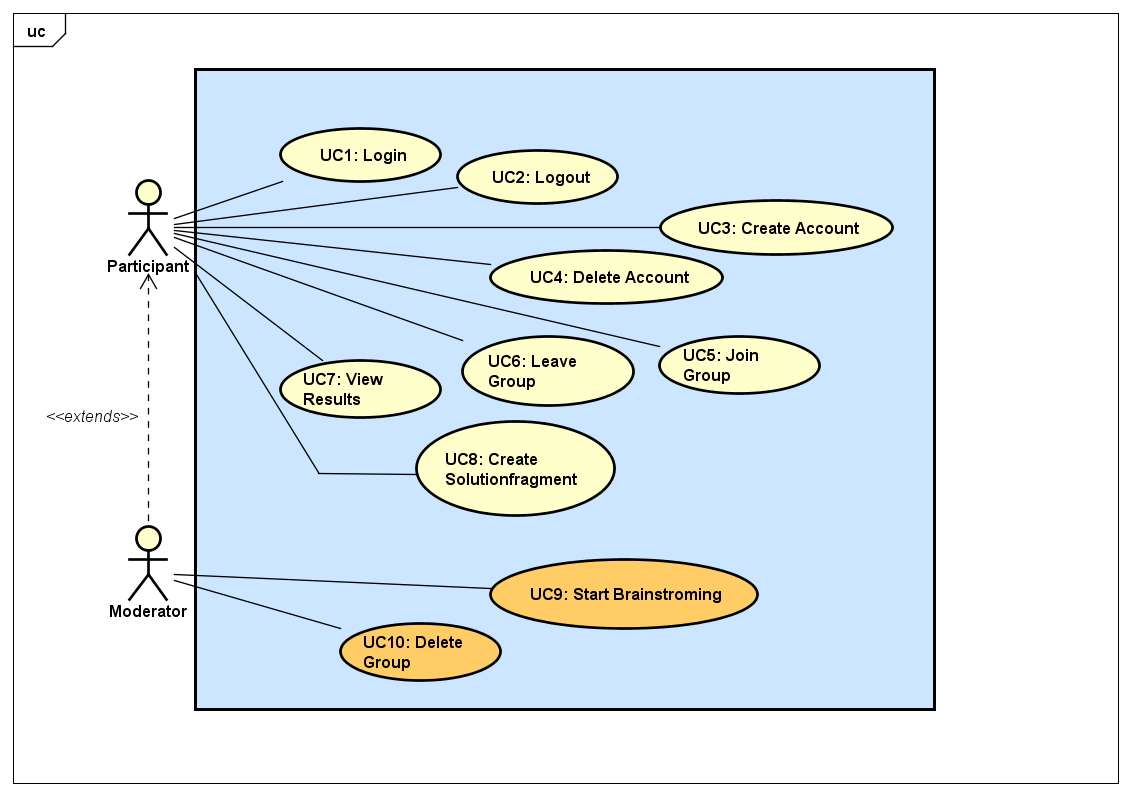
\includegraphics[width=1\linewidth]{img/anforderungen/UC-Methode635}
	\caption{Use-Case-Diagramm}
	\label{fig:ucmethode-635}
\end{figure}

Jeder Use-Case hat den nachfolgend kurz (\textit{briefly}) beschriebenen  Funktionsumfang. Die Hauptaktivitäten UC7-9 sind am Schluss \textit{fully-dressed} beschrieben.

\begin{basedescript}{%
		\desclabelstyle{\multilinelabel}
		\desclabelwidth{4.5cm}}
	\item[\textit{UC1: }Login] Als Participant möchte ich mich mit Benutzernamen und Passwort in das System einloggen können.
	\item[\textit{UC2: }Logout] Als eingeloggter Participant will ich mich ausloggen, sodass das Startfenster wieder erscheint.
	\item[\textit{UC3: }Create Account] Als Benutzer der Applikation möchte ich mich registrieren können.
	\item[\textit{UC4: }Delete Account] Als Benutzer will ich meinen erstellten Account wieder löschen können.
	\item[\textit{UC5: }Join Group] Als Participant will ich einer bereits existierenden Gruppe beitreten können.
	\item[\textit{UC6: }Leave Group] Als Participant will eine beigetretene Gruppe verlassen können.
	\item[\textit{UC7: }View Results] Als Participant will ich, nachdem eine Brainstorming Session durchgeführt wurde, das Resultat meiner Gruppe einsehen können.
	\item[\textit{UC8: }Create\\Solutionfragment] Als Participant will ich während einer Brainstorming Session ein Lösungsfragment erstellen und einreichen können. 
	\item[\textit{UC9: }Start \\Brainstorming] Als Moderator will ich eine Brainstorming Session starten.
	\item[\textit{UC10: }Create Group] Als Moderator will ich eine Gruppe erstellen können. 
	\item[\textit{UC11: }Delete Group] Als Moderator will ich eine Gruppe löschen können.
\end{basedescript}

\paragraph{Fully-Dressed Use-Cases}


\paragraph{Abuse-Cases}
%Abuse cases?
Um einem Missbrauch der Applikation entgegenzuwirken, sind neben den Use-Cases auch Abuse-Cases definiert. Diese helfen, mit unangebrachtem Inhalt und unangebrachter Verwendung umzugehen.
\begin{basedescript}{%
		\desclabelstyle{\multilinelabel}
		\desclabelwidth{4.5cm}}
	\item[\textit{AC1: }Unangebrachte Lösungsfragmente] Ein Participant könnte unangebrachte Inhalte in einer Gruppe hinzufügen. Um dies zu verhindern, könnte eine die Applikation um eine Funktion erweitert werden, die es dem Moderator erlaubt, Benutzer auszuschliessen.
\end{basedescript}

%Sequence diagram
\paragraph{Sequenzdiagramm}
Der Ablauf der Kernlogik ist der Abbildung \ref{fig:seq-methode635} zu entnehmen. Darin ist der Prozess vom Erstellen der Gruppe (UC10) bis zum Abschliessen der Brainstorming Session modelliert.
\begin{figure}[h]
	\centering
	\makebox[\textwidth][c]{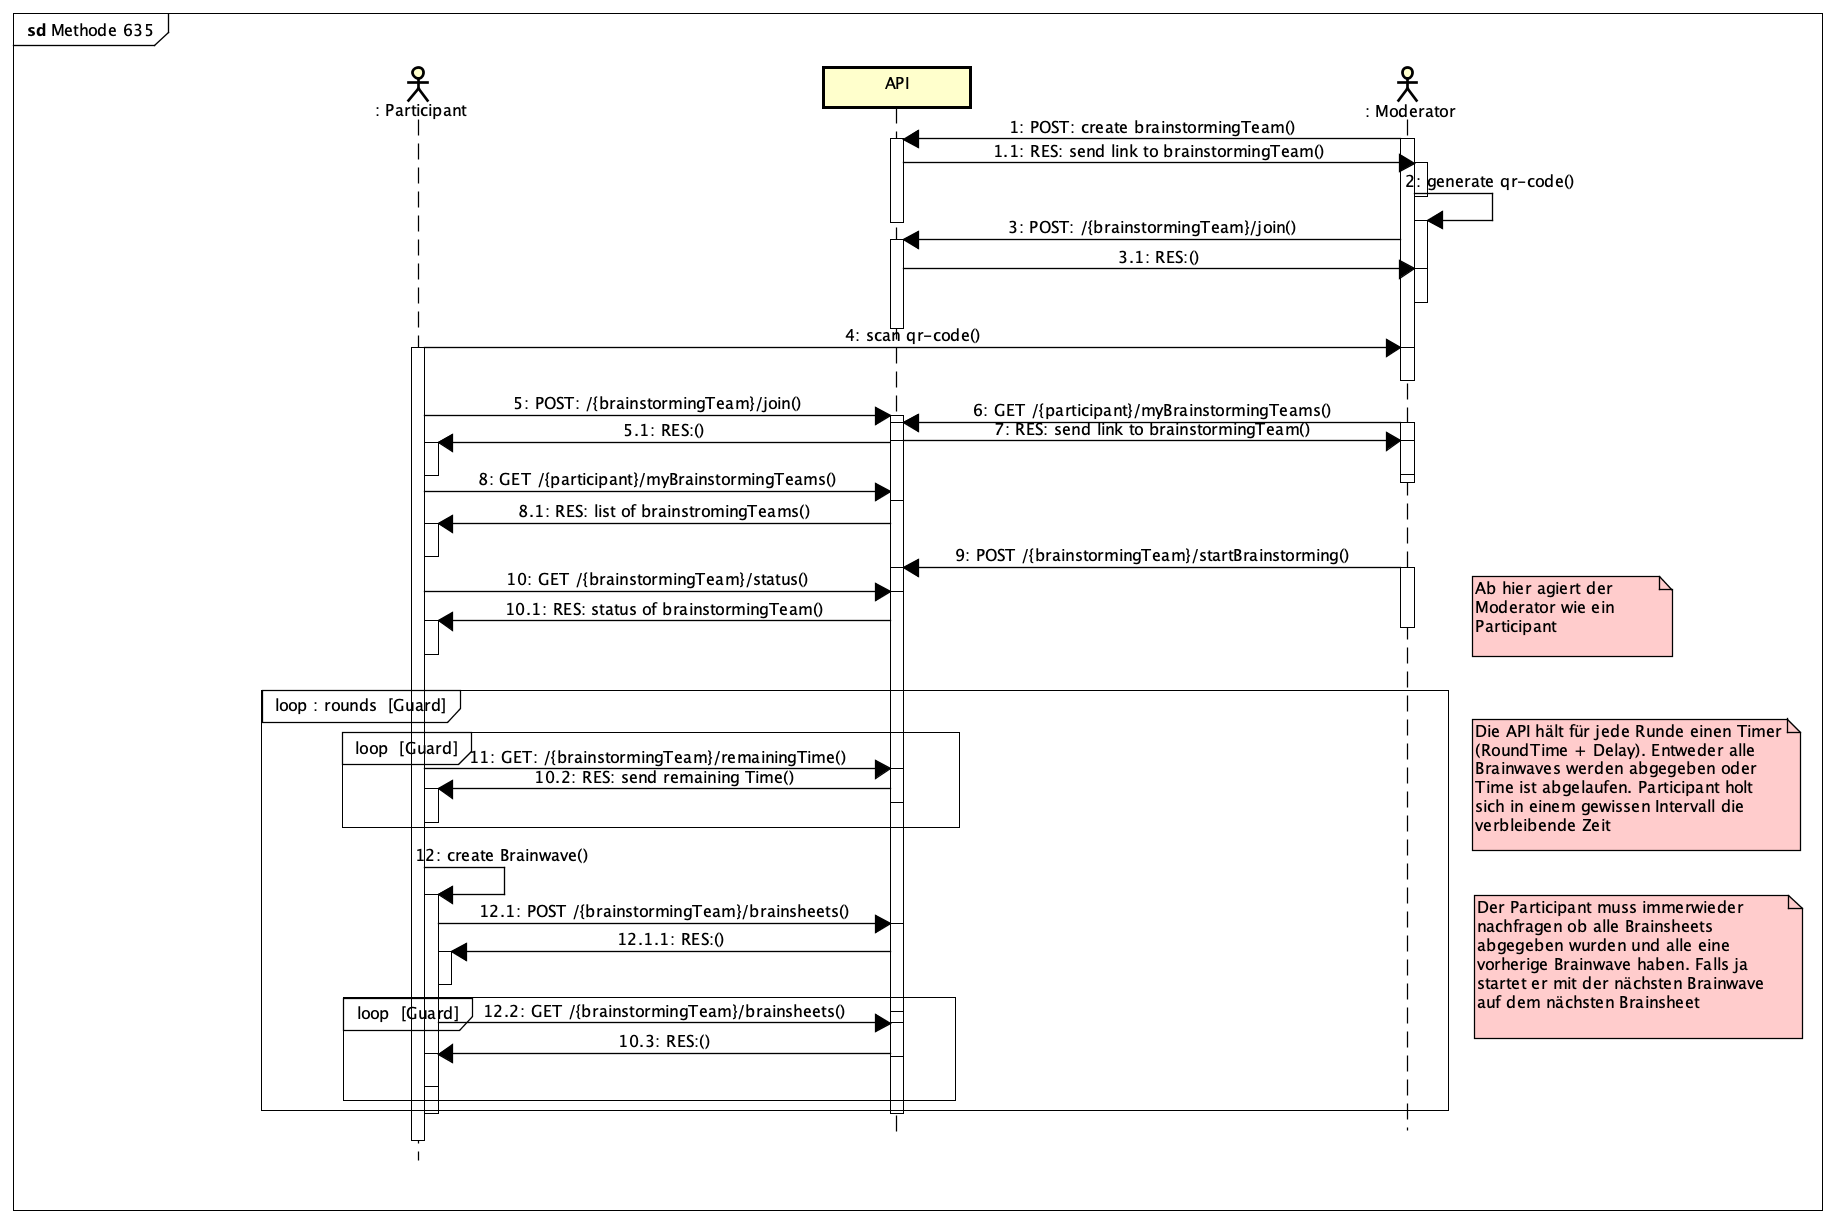
\includegraphics[width=1.2\linewidth]{img/anforderungen/Seq-Methode635}}
	\caption{Sequenzdiagramm}
	\label{fig:seq-methode635}
\end{figure}


\subsubsection{Nicht-Funktionale Anforderungen}
Beim Thema Nicht-Funktionale Anforderungen halten wir uns an die Standards ISO 9126\cite{ISO9126} bzw. dessen Nachfolger ISO 25010\cite{ISO9126_ISO25010}. Beide ISO-Normen sind sich sehr ähnlich und liefern eine gute Checkliste für jegliche Art von Systemanforderungen.

\begin{figure}[h]
	\centering
	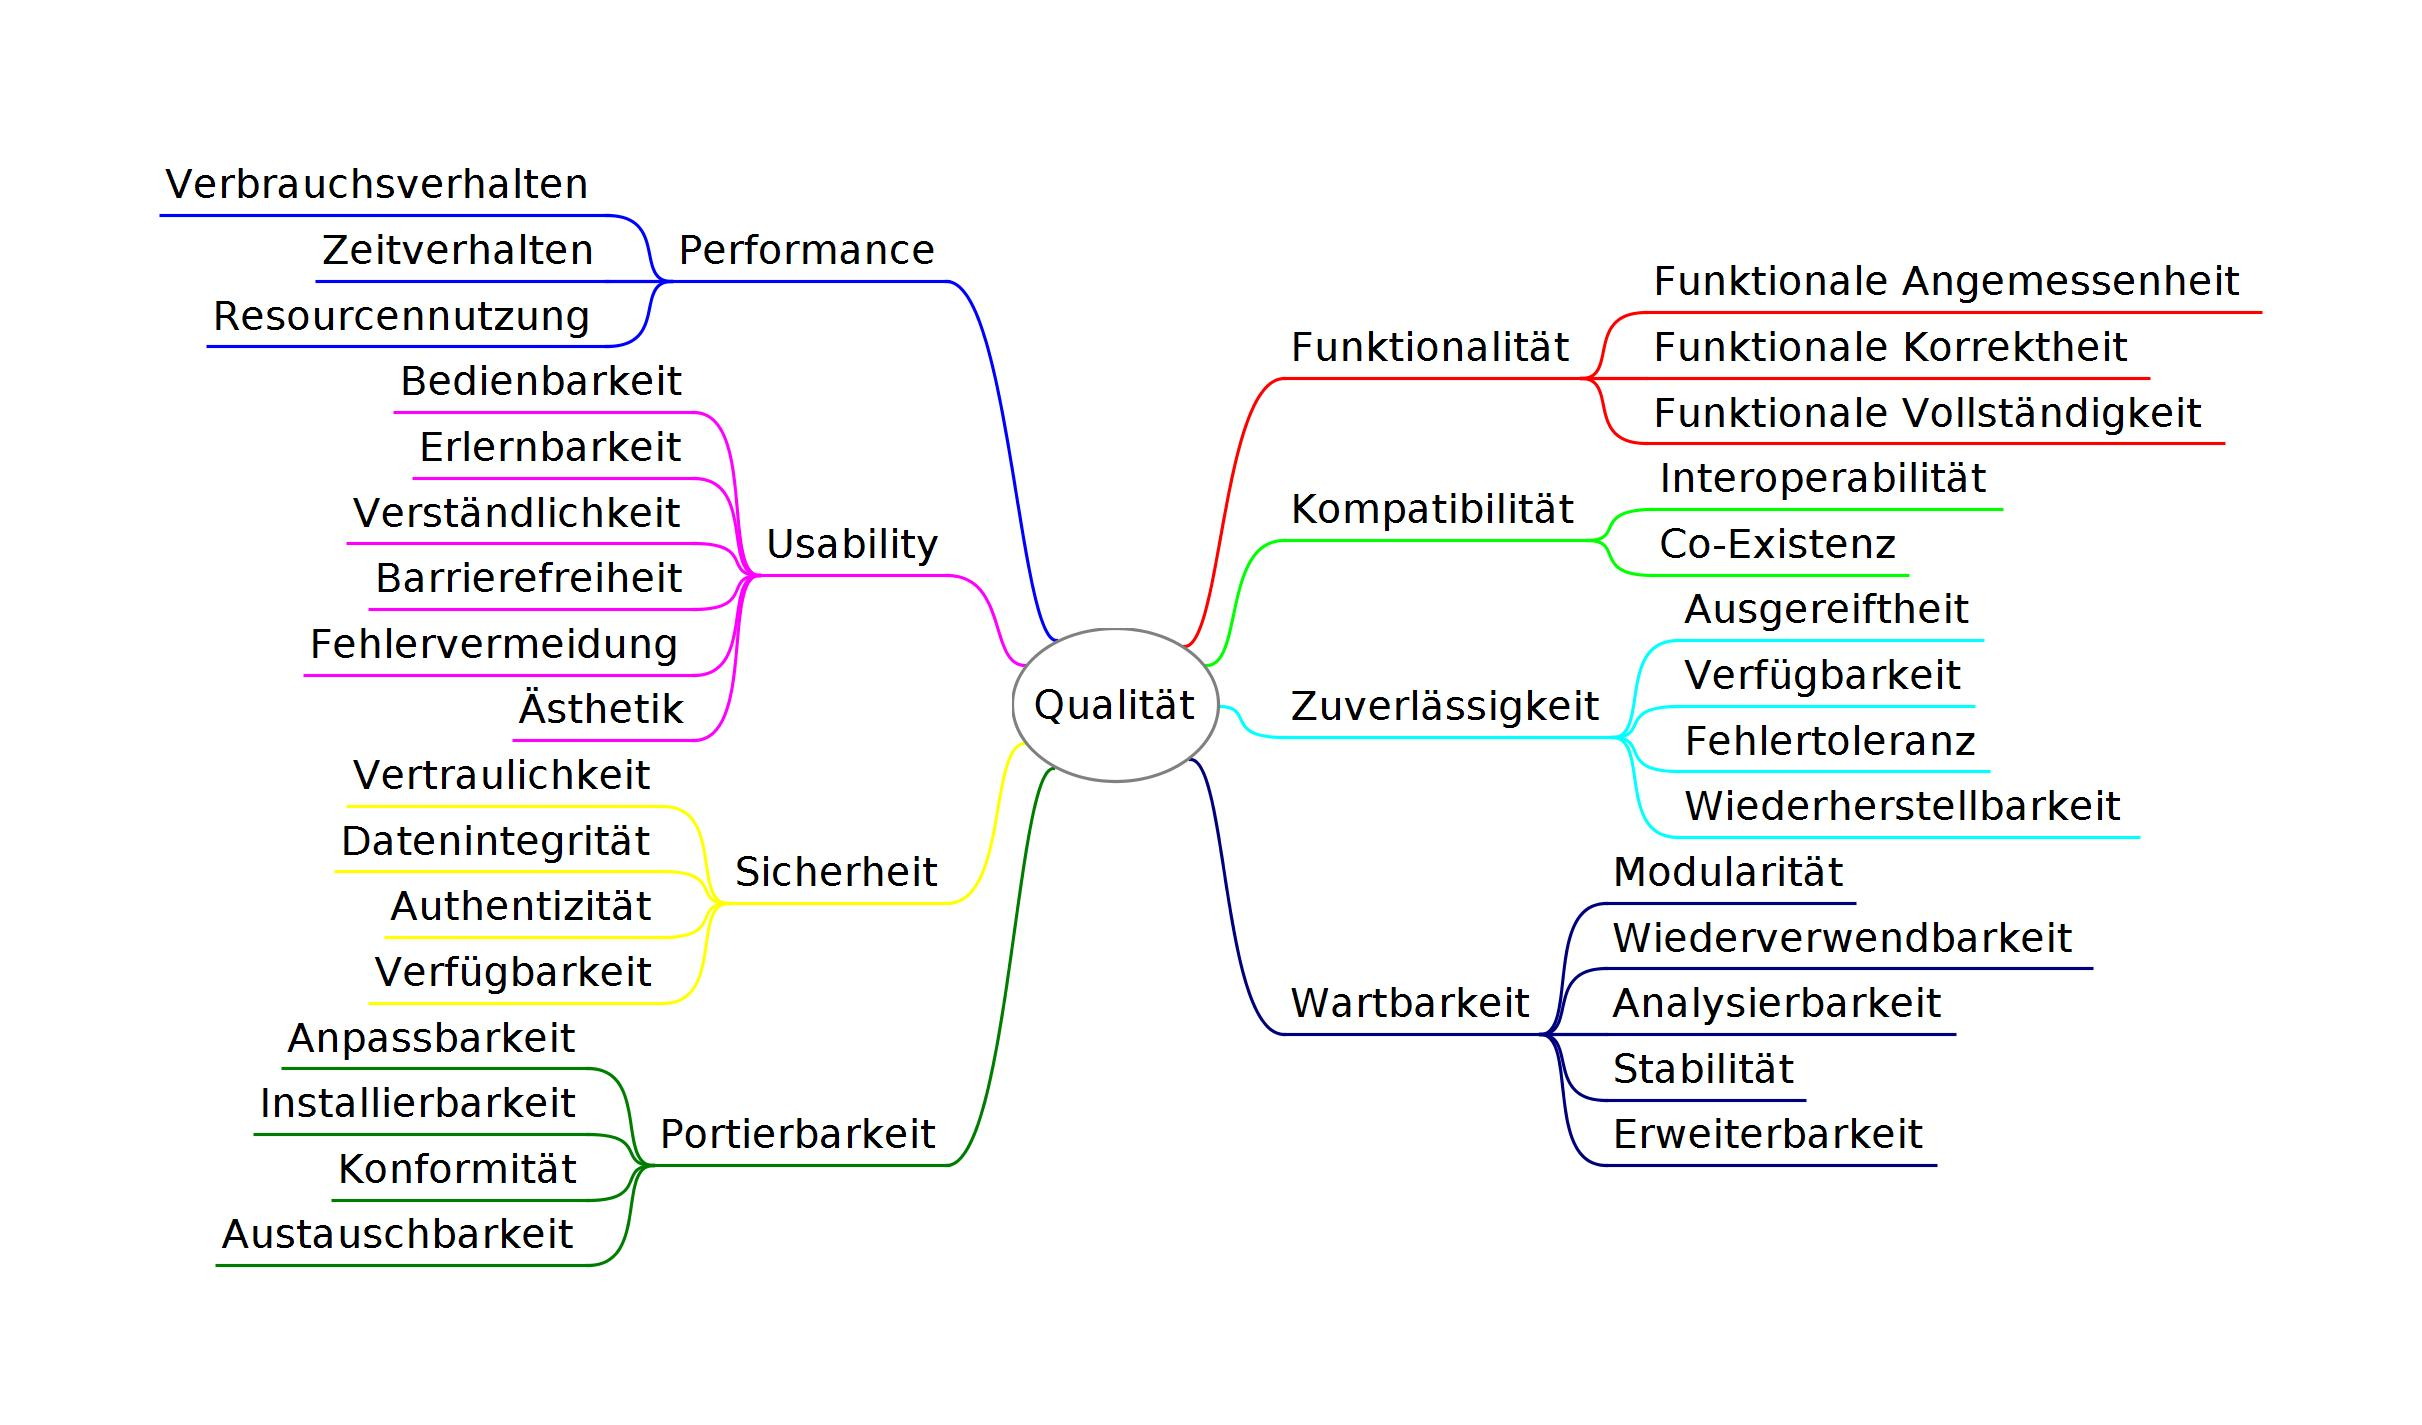
\includegraphics[width=1\linewidth]{img/anforderungen/quality}
	\caption[Anforderungskategorien nach ISO 25010]{Anforderungskategorien nach  ISO 25010}
	\label{fig:ISO 25010}
\end{figure}

%TODO Bild Link: https://blog.seibert-media.net/blog/2018/05/14/qualitaet-funktionale-und-nichtfunktionale-anforderungen-in-der-software-entwicklung/

Diese Normen sind sehr umfangreich gestaltet. Wir werden uns daher auf die, für uns, wichtigsten Anforderungen konzentrieren. Um genaue und erfüllbare nicht-funktionale Anforderungen zu definieren, müssen die SMART-Kriterien \cite{SMART} erfüllt sein. 

\begin{description}[leftmargin=!,labelwidth=\widthof{\bfseries Wiederverwendbarkeit}]
	\item[Ressourcennutzung] Die internen Ressourcen Kamera, Dateisystem dürfen nur bei effektivem Bedarf benützt werden. Die CPU-Ressourcen\-nutzung darf im Durchschnitt pro Minute maximal zu 40\% in Anspruch genommen werden.\footnote{Referenzsystem Android: Huawei P10 mit Android Version 8.0.0 mit Hisilicon Kirin 960 CPU und 4GB RAM}\footnote{Referenzsystem iOS: iPhone 6 mit iOS Version 12 mit Dual-core 1.4 GHz Typhoon CPU und 1GB RAM}
	
	\item[Bedienbarkeit] Wenn eine Aktion länger als 1-2s geht, soll dem User ein Wartesymbol angezeigt werden. 
	
	\item[Ästhetik] Die Benutzeroberflächen der Applikation sind so gestaltet, dass die Elemente wiedererkennbar sind (Buttons haben gleichen Stil, leere Textfelder haben Platzhalter). 
	
	\item[Vertraulichkeit] Die Daten einer Brainstorming Session können nur von der zugehörigen Gruppe eingesehen werden. 
	
	\item[Anpassbarkeit] Die Anpassung bestehender oder Integration neuer Brain\-storming-Methoden muss gewährleistet sein.
	
	\item[Installierbarkeit] Die Installation der Applikation auf einem Endgerät erfolgt durch das Ausführen eines *.apk oder *.app. Dieser Prozess soll unter 1 Minute geschehen.
	
	\item[Co-Existenz] Sollte zu einem späteren Zeitpunkt entschieden werden ein Web-Frontend zu programmieren, muss dieses co-existent mit der Xamarin Applikation existieren können.
	
	\item[Wiederherstellbarkeit] Im Falle eines fehlerhaften Features, muss es innerhalb eines Werktages möglich sein, die Applikation wieder auf den letzten funktionierenden Stand zurück zu holen und erneut zu deployen.	
	
	\item[Wiederverwendbarkeit] Die Auswertung von 'Duplicated Code' in SonarQube soll unter 8\% liegen. Dies deutet auf eine hohe Wiederverwendbarkeit hin, denn ansonsten müsste der Code kopiert werden. 
	
	%TODO: Referenz auf Use Cases
	\item[Analysierbarkeit] Das Ausführen eines Use-Cases muss durch Analyse von Logfiles erkennbar sein.
\end{description}

\newpage

\subsection{Domainanalyse}

Das Domain-Modell besteht grob aus zwei Teilen: den Benutzern und der Brainstorming Methodik. 

Dabei bilden mehrere Participants ein \textit{Brainstorming Team}. Diese wird von einem der Participants, dem \textit{Moderator}, gegründet.  Das Team hat die Möglichkeit, ein oder mehrere \textit{Brainstorming Findings} zu erarbeiten. Dies entspricht einer gesamten Durchgang der Methode. Der Moderator erstellt diese und hat die Möglichkeit, die Anzahl von Ideen sowie die erste Rundenzeit zu konfigurieren. Jede weitere Runde wird um eine Minute verlängert.

Das \textit{Brainsheet} entspricht einem physikalischem Blatt, das herumgegeben wird. In der Standardkonfiguration 635 existieren also 6 Sheets (weil 6 Teilnehmer dabei sind).

Eine \textit{Brainwave} ist das Produkt jedes Participants am Ende einer Runde. Es gehört in ein Brainsheet, das jede Runde an den nächsten Participant weitergegeben wird. In der Standardkonfiguration besteht eine Brainwave aus 3 Ideen (6\textbf{3}5).

Die \textit{Idea} ist ein effektiv erarbeiteter Teil einer Brainwave. Im Normalfall ist eine Idee simpler Text (\textit{NoteIdea}), wobei weitere Typen von Ideen (Bild, Weblink und Zeichnung) durch das verwendete Design erdenklich sind. 
\begin{figure}[h]
	\centering
	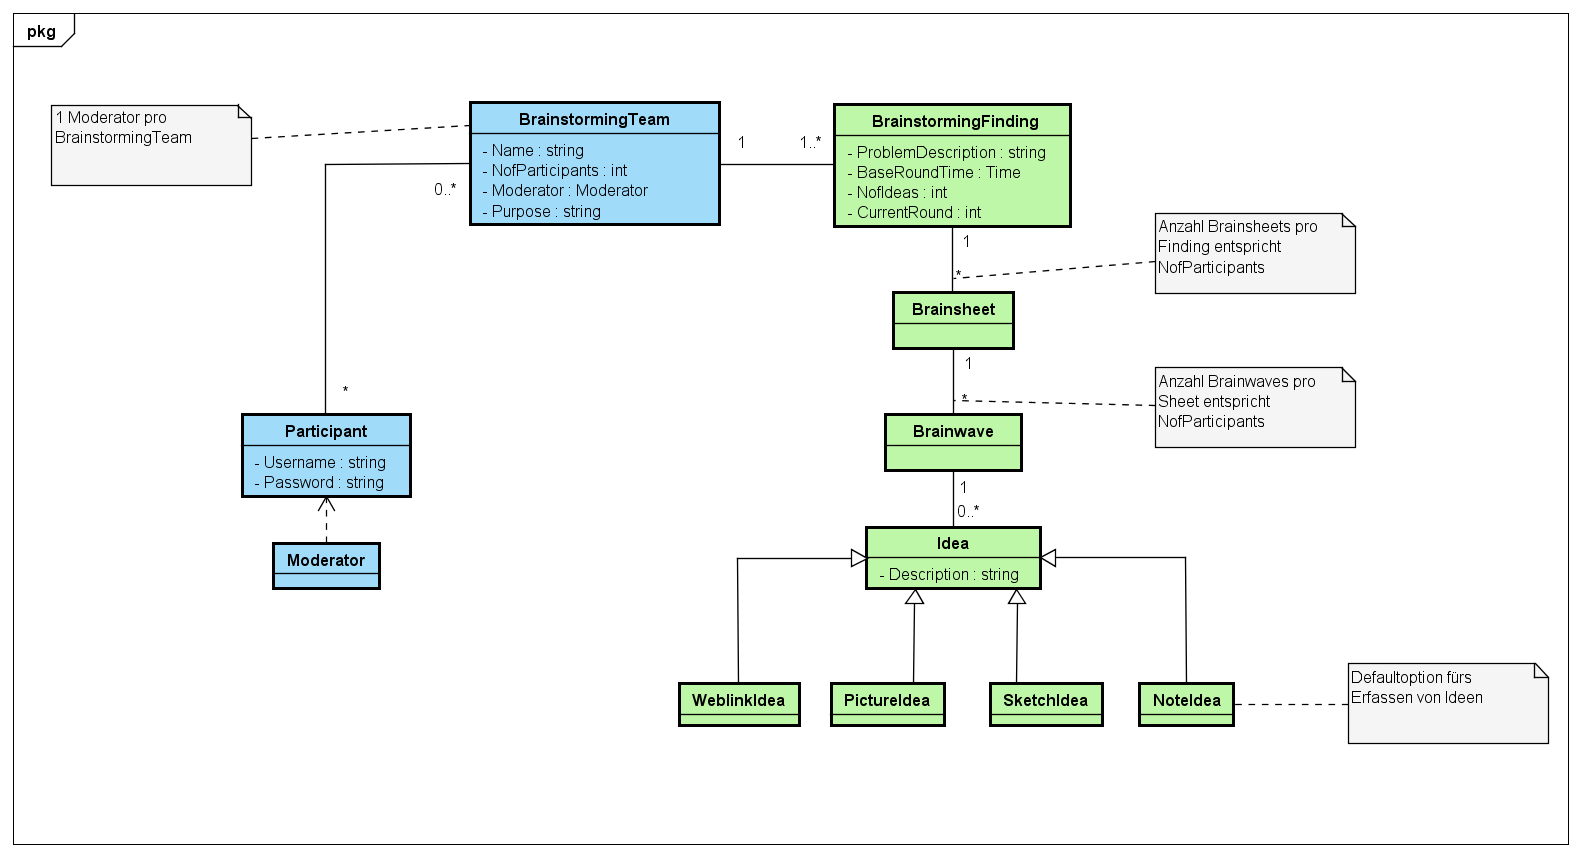
\includegraphics[width=1\linewidth]{img/domain-analyse/DomainModell-Methode635}
	\caption{Domain Modell BrainingOutOfBox}
	\label{fig:domainmodell-methode635}
\end{figure}

\newpage


\subsection{Ergebnisse}

\subsection{Schlussfolgerungen}
\subsubsection{Ergebnisbewertung}
\subsubsection{Ausblick}